\begin{question}[ID=xavyvn,type=exam]{10}
Consider the restaurant game from class where Xavier and Yvonne restaurant's
competing for customers where Xavier's quantity sold is $Q_x = 44 - 2P_x + P_y$
and Yvonne's quantity sold is $Q_y = 44 - 2P_y + P_x$ with Xavier setting his
price at $P_x$, and Yvonne setting hers at $P_y$. \\
But now instead of having identical costs, suppose that Yvonne's cost per meal
is lowered to \vary{\$2}{\$4} and Xavier's cost per meal is increased to
\vary{\$8}{\$12}. \\
Xavier's best response rule is given by:
$$ BR_x(P_y) = \frac{1}{4} P_y + \vary{15}{17} $$
Yvonne's best response rule is given by:
$$ BR_y(P_x) = \frac{1}{4} P_x + \vary{12}{13} $$
\begin{tasks}
  \task 
  Solve for any Nash equilibria in this pricing game.
  Explain why they are stable.
  \PrintSolutionsTF{
  \fbox{
    \parbox{\linewidth}{
    SOLUTION
    \vary
    {
    \begin{center}
    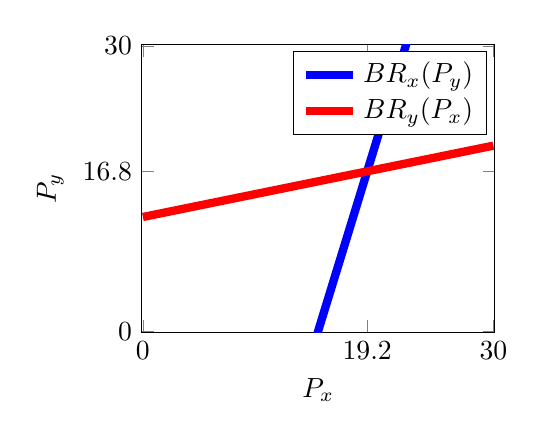
\begin{tikzpicture}
      \begin{axis}[
        width=.5\textwidth,
        xlabel={$P_x$},
        ylabel={$P_y$},
        xmin=-0.1, xmax=30.1,
        ymin=-0.1, ymax=30.1,
        xtick={0,19.2,30},
        ytick={0,16.8,30},
        ]
        \addplot [
        domain=0:30,
        line width=3pt,
        color=blue,
        ] 
        {4*x - 44 - 2*8};
        \addlegendentry{\(BR_x(P_y)\)}
        \addplot [
        domain=0:30,
        line width=3pt,
        color=red,
        ] 
        {11 + .5*2 + .25*x};
        \addlegendentry{\(BR_y(P_x)\)}
      \end{axis}
    \end{tikzpicture}
    \end{center}
    }
    {
    \begin{center}
    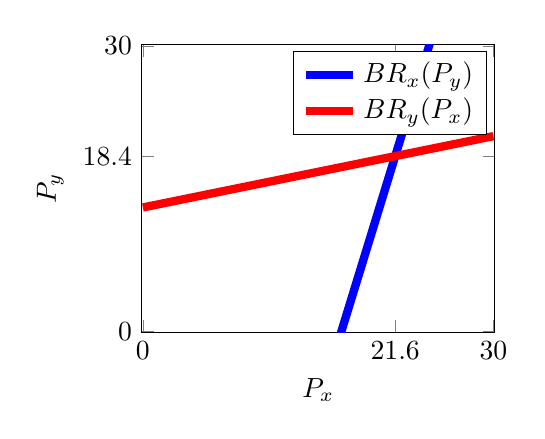
\begin{tikzpicture}
      \begin{axis}[
        width=.5\textwidth,
        xlabel={$P_x$},
        ylabel={$P_y$},
        xmin=-0.1, xmax=30.1,
        ymin=-0.1, ymax=30.1,
        xtick={0,21.6,30},
        ytick={0,18.4,30},
        ]
        \addplot [
        domain=0:30,
        line width=3pt,
        color=blue,
        ] 
        {4*x - 44 - 2*12};
        \addlegendentry{\(BR_x(P_y)\)}
        \addplot [
        domain=0:30,
        line width=3pt,
        color=red,
        ] 
        {11 + .5*4 + .25*x};
        \addlegendentry{\(BR_y(P_x)\)}
      \end{axis}
    \end{tikzpicture}
    \end{center}
    }
    In NE, $BR_x(P_y) = P_x$ and $BR_y(P_x) = P_y$.
    \begin{align*}
      P_x & = \frac{1}{4}(\frac{1}{4}P_x + \vary{12}{13}) + \vary{15}{17} \\
      P_x & = \frac{1}{16}P_x + \frac{\vary{12}{13}}{4} + \vary{15}{17} \\
      \frac{15}{16} P_x & = \vary{18}{20.25} \\
      P_x^* & = \vary{19.2}{21.6}
    \end{align*}
    Plug $P_x^*$ into $BR_y()$:
    \begin{align*}
      P_y & = \frac{1}{4} (\vary{19.2}{21.6}) + \vary{12}{13} \\
      P_y^* & = \vary{16.8}{18.4}
    \end{align*}
    ($P_x =$ \vary{19.2}{21.6}, $P_y = $ \vary{16.8}{18.4})
    is the only NE in this game because it is the only set of prices
    both players' best response rules intersect.
    }}
  }{
    \vspace{5cm}
  }
\end{tasks}
\end{question}

\begin{question}[ID=vlccs,type=exam]
Crude oil is transported across the globe in enormous tanker ships called
Very Large Crude Carriers (VLCCs). 
% By 2001, more than 92\% of all new VLCCs were built in South Korea and Japan.
Assume that the price of new VLCCs (in millions of dollars) 
is determined by the function $P = 166 - Q$,
where $Q = q_{Korea} + q_{Japan}$. 
(That is, assume that only Japan and Korea produce VLCCs, so they are a duopoly.)
Assume that the cost of building each ship is \$\vary{7}{9} million in both Korea
and \$\vary{10}{14} million in Japan. 
That is, $c_{Korea} = \vary{7}{9}$, $c_{Japan} = \vary{10}{14}$,
where the per-ship cost is measured in millions of dollars.
\begin{tasks}
  \task (\points{4}) Solve for \textit{Korea}'s best response rule to Japan's price.
  \task (\points{4}) Solve for \textit{Japan}'s best response rule to Korea's price.
  \task (\points{4}) Graph the best-responses with the x-axis as Korea's price
  and the y-axis as Japan's price.
  \task (\points{4}) Solve for all Nash Equilibria. Explain why they are stable.
\end{tasks}
\begin{solution}
  \begin{tasks}
    \task $BR_{Korea}(q_{Japan}) = \frac{166-q_{Korea}-\vary{7}{9}}{2} = \vary{79.5}{78.5}-0.5q_{Korea}$
    \par\noindent\rule{\linewidth}{0.4pt}
    4 points if correct answer, 3 if correct setup shown in work but algebra mistakes,
    2 points if incorrect answer and missing work or incorrect setup,
    1 point if wrong answer and no work/justification.
    \task $BR_{Japan}(q_{Korea}) = \frac{166-q_{Japan}-\vary{10}{14}}{2} = \vary{78}{76}-0.5q_{Japan}$
    \task Graph: \\
    \vary{
    \begin{center}
    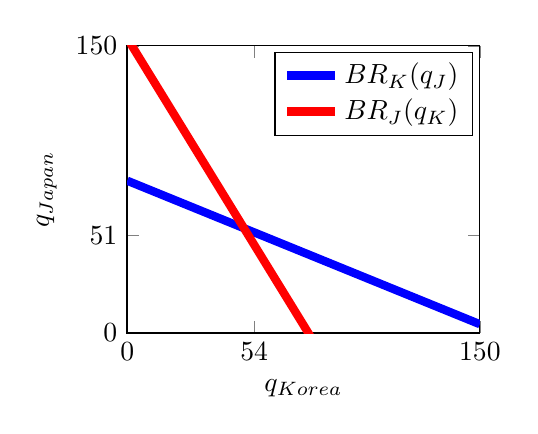
\begin{tikzpicture}
      \begin{axis}[
        width=.5\textwidth,
        xlabel={$q_{Korea}$},
        ylabel={$q_{Japan}$},
        xmin=-0.1, xmax=150,
        ymin=-0.1, ymax=150,
        xtick={0,54,150},
        ytick={0,51,150},
        ]
        \addplot [
        domain=0:150,
        line width=3pt,
        color=blue,
        ] 
        {79.5-0.5*x};
        \addlegendentry{\(BR_K(q_J)\)}
        \addplot [
        domain=0:150,
        line width=3pt,
        color=red,
        ] 
        {154-2*x};
        \addlegendentry{\(BR_J(q_K)\)}
      \end{axis}
    \end{tikzpicture}
    \end{center} 
    }{
    \begin{center}
    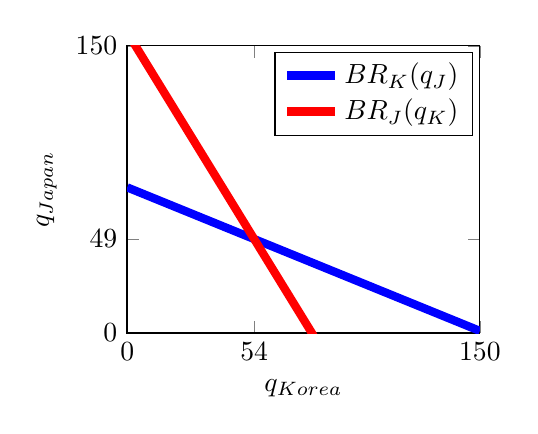
\begin{tikzpicture}
      \begin{axis}[
        width=.5\textwidth,
        xlabel={$q_{Korea}$},
        ylabel={$q_{Japan}$},
        xmin=-0.1, xmax=150,
        ymin=-0.1, ymax=150,
        xtick={0,54,150},
        ytick={0,49,150},
        ]
        \addplot [
        domain=0:150,
        line width=3pt,
        color=blue,
        ] 
        {76-0.5*x};
        \addlegendentry{\(BR_K(q_J)\)}
        \addplot [
        domain=0:150,
        line width=3pt,
        color=red,
        ] 
        {157-2*x};
        \addlegendentry{\(BR_J(q_K)\)}
      \end{axis}
    \end{tikzpicture}
    \end{center} 
    }
    \par\noindent\rule{\linewidth}{0.4pt}
    4 if graph matches key.
    3 if wrong but makes sense from previous work or obvious minor error.
    2 if wrong but well labelled and seems plausible.
    1 if unlabelled and unclear how it fits with student's work.
  \task
    The only NE is ${q_K = \vary{54}{54}, q_J =  \vary{51}{49}}$
    These quantities are stable because if for example,
    Korea sets a lower price, they would earn less profit.
    Same for Japan.
    \par\noindent\rule{\linewidth}{0.4pt}
    4 points if numbers are correct explained. 
    3 if numbers are off but match work above and well explained. 
    2 if wrong numbers and doesn't make sense with previous work or explanation. 
    1 if wrong answers with no work/explanation.
  \end{tasks}
\end{solution}
\end{question}